\let\cleardoublepage\clearpage
\begin{appendices}
\chapter{RDF-Doctor Grammar}
\label{ch:appendix}
% Applies only when you use it
\lstset{
    basicstyle=\color{black}\ttfamily,%
    breaklines=true,%                                      allow line breaks
    moredelim=*[s][\color{black}\ttfamily]{options}{\}},%  options in black (until trailing })
    commentstyle={\color{gray}\itshape},%                  gray italics for comments
    morecomment=[l]{//},%                                  define // comment
    emph={%
        STRING%                                            literal strings listed here
        },emphstyle={\color{blue}\ttfamily},%              and formatted in blue
    alsoletter={:,|,;},%
    morekeywords={:,|,;},%                                 define the special characters
    keywordstyle={\color{black}},%                         and format them in black
}

\begin{lstlisting}
grammar Turtle;
@parser::members { 
// Add member functions to check Namespace declaration
public List<String> symbols = new ArrayList<String>();
boolean isExistNS(String in ) { 
// Custom constructor
	boolean foundNS = false ; 
		if(symbols.contains(in.split(":")[0]+':')) foundNS=true;
	return foundNS;
}
}
// Start of grammar rules with 'start' root node
start
    : statement*  EOF
    ;
// statement is either a prefix declaration of a triple
statement
    : directive
    |  IRIREF IRIREF IRIREF  graphLabel '.' {notifyErrorListeners("Turtle is not NQOUDS");}
    | triple '.'
    | triple {notifyErrorListeners("Missing '.' at the end of a triple");}
    | triple ',' {notifyErrorListeners("Bad end of a triple with ','");}
    | triple ';' {notifyErrorListeners("Bad end of a triple with ';'");}
    | triple ('.')+ ('.')+ {notifyErrorListeners("Too many DOT");}
    | errors		
    ;
directive
    : sparqlPrefix
    | sparqlBase 
    | prefixID   
    | base
    | unkonwnDecl
    | sparqlPrefix '.' {notifyErrorListeners("Extraneous '.' at the end of SPARQL prefix directive");}
    | sparqlBase '.' {notifyErrorListeners("Extraneous '.' at the end of SPARQL base directive");}
    ;
errors	
    : iri '=' iri '.' {notifyErrorListeners("'=' sign cannot be used in Turtle");}
 	| iri '<=' iri '.'  {notifyErrorListeners("'<=' symbol cannot be used in Turtle");}
    | iri '=>' iri '.'  {notifyErrorListeners("'=>' symbol cannot be used in Turtle");}
 	| (iri '.')+ (iri '.')+  triple '.' {notifyErrorListeners("N3 paths cannot be used in Turtle");}
    | (iri '.')+ (iri '.')+  triple  {notifyErrorListeners("N3 paths cannot be used in Turtle");}
    | iri '^'  triple '.' {notifyErrorListeners("N3 paths cannot be used in Turtle");}
    | '@forAll' iri '.' {notifyErrorListeners(" '@forAll' cannot be used in Turtle ");}
    | '@forSome' iri '.' {notifyErrorListeners(" '@forSome' cannot be used in Turtle ");}
    | ('a'|CHARS)* '@a' ('a'|CHARS)* '.' {notifyErrorListeners(" '@a' cannot be used in Turtle ");}
    ;
 graphLabel
 	: 	IRIREF | BLANK_NODE_LABEL
 	;
 unkonwnDecl 	
    : '@keywords' ('a'|CHARS)*  '.' {notifyErrorListeners("@keywords is unkown directive in Turtle");}
	;	
prefixID
    : '@prefix' CHARS '.' ':' IRIREF '.' {notifyErrorListeners("Prefix-label cannot end with '.' ");}
    | '@prefix' '.' CHARS ':' IRIREF '.' {notifyErrorListeners("Prefix-label cannot start with '.' ");}
    | '@prefix' ':' IRIREF '.' { symbols.add(":");} { System.out.println(":" + $IRIREF.text);} 
    | '@prefix' PNAME_NS  IRIREF '.' {symbols.add($PNAME_NS.text);}  { System.out.println($PNAME_NS.text + $IRIREF.text);} 
    | '@prefix' PNAME_NS IRIREF ('.')+ ('.')+ {notifyErrorListeners("Too many DOT ");}
    | PNAME_NS IRIREF '.' {notifyErrorListeners("Missing Prefix keyword, use '@prefix'");}
    | '@prefix'   IRIREF '.' {notifyErrorListeners("Missing Prefix-label in Prefix directive");}
    | '@prefix' CHARS*  IRIREF '.'  {notifyErrorListeners("Missing ':' in Prefix directive");}
    ;
base
    : '@base' IRIREF '.'
    | '@base' IRIREF ('.')+ ('.')+ {notifyErrorListeners("Too many DOT ");}
    ;
sparqlBase
    : KW_BASE  IRIREF 
    | '@BASE'   IRIREF '.'  {notifyErrorListeners("incorrect syntax form of base directive");}
    ;
sparqlPrefix
    : KW_PREFIX CHARS '.' ':' IRIREF  {notifyErrorListeners("Prefix-label cannot end with '.' ");}
    | KW_PREFIX '.' CHARS ':' IRIREF  {notifyErrorListeners("Prefix-label cannot start with '.' ");}
    | KW_PREFIX PNAME_NS IRIREF
    | KW_PREFIX ':' IRIREF
    | PNAME_NS IRIREF {notifyErrorListeners("Missing Prefix keyword, use 'PREFIX'");}
    | KW_PREFIX  IRIREF  {notifyErrorListeners("Missing Prefix-label in Prefix directive");}
    ;
KW_BASE 
    : B A S E 
    ;
KW_PREFIX 
    : P R E F I X 
    ;
triple
    : subject predicateObjectList
    | blankNodePropertyList predicateObjectList?
    | subject ':' object 
    | subject verb {notifyErrorListeners("Object of a triple is missing");}
    ;
predicateObjectList
    : verb objectList (';' verb objectList)*
    | verb objectList (';' verb objectList)* ('.')+ {notifyErrorListeners("Too many dots ");}
    | verb objectList (';' verb )* {notifyErrorListeners("Object of a triple is missing");}
    | verb  (';' verb objectList)* {notifyErrorListeners("Object of a triple is missing");}
    | verb objectList (';' verb objectList)* (';' verb )+ (';' verb objectList)* {notifyErrorListeners("Object of a triple is missing");}
    ;
objectList
    : object (',' object)*
    ;
verb
    :   'a' 
    | predicate
    | 'is' predicate 'of' {notifyErrorListeners("'is .. of' pattern is not used in Turtle");}
    | 'A' {notifyErrorListeners("'A' cannot be used as predicate, it should be replaced with 'a'");}
    | BooleanLiteral {notifyErrorListeners("Predicate cannot be a Boolean value");}
    | NumericLiteral  {notifyErrorListeners("Predicate cannot be a number");}
    | literal {notifyErrorListeners("Predicate cannot be a literal");}
    | BlankNode {notifyErrorListeners("Predicate cannot be a blank node");}
    ;
subject
    : iri
    | BlankNode
    | BlankNode  '.' {notifyErrorListeners("Blank Node cannot be followed by '.'");}
    | 'a' {notifyErrorListeners("'a' cannot be used as a subject");}
    | BooleanLiteral {notifyErrorListeners("Subject cannot be a Boolean value");}
    | NumericLiteral  {notifyErrorListeners("Subject cannot be a number");}
    | rdfLiteral   {notifyErrorListeners("Subject cannot be a string");}
    | collection
    | '{' triple '.' '}' {notifyErrorListeners("{ } pattern cannot be used in Turtle");}
    | '{' triple '}' {notifyErrorListeners("{ } pattern cannot be used in Turtle");} 
    ;
predicate
    : iri
    ;
object
    : iri
    | BlankNode
    | collection
    | blankNodePropertyList
    | badBlankNodePropertyList  {notifyErrorListeners("incorrect form of a blank node list");}
    | literal
    | 'a' {notifyErrorListeners("'a' cannot be used as an object");}   
    ;
literal
    : rdfLiteral
    | NumericLiteral
    | BooleanLiteral
    | BadLiteral {notifyErrorListeners("incorrect form of a Literal");}
    ;
blankNodePropertyList
    : '[' predicateObjectList ']'
    ;
badBlankNodePropertyList   
	: '[' predicateObjectList '.' ']'
	;
collection
    : '(' object* ')'
    ;
NumericLiteral
    : INTEGER | DECIMAL | DOUBLE
    ;
rdfLiteral
    : BAD_STRING_LITERAL_LONG_QUOTE_WITH_OPEN_QUOTES  (LANGTAG | '^^' iri)?  {notifyErrorListeners("incorrect form of long literal with uncolsed qoutes");}
    | BAD_STRING_LITERAL_LONG_QUOTE_TOO_MANY (LANGTAG | '^^' iri)? {notifyErrorListeners("incorrect form of long literal with 4 qoutes");}
    | BAD_STRING_LITERAL_LONG_SINGLE_QUOTE_TOO_MANY (LANGTAG | '^^' iri)? {notifyErrorListeners("incorrect form of long literal with 4 qoutes");}
    | String  BAD_LANGTAG_AS_NUMBER  {notifyErrorListeners("Language tag cannot be a numeric value");}
    | String '^' iri {notifyErrorListeners("Missing '^' Character");}
    | String LANGTAG '^^' iri {notifyErrorListeners("incorrect form of a Literal");}
    | String '^^' iri LANGTAG {notifyErrorListeners("incorrect form of a Literal");}  
    | (BAD_STRING_LITERAL_LONG_SINGLE_QUOTE | BAD_STRING_LITERAL_LONG_QUOTE ) (LANGTAG | '^^' iri)?  {notifyErrorListeners("incorrect quotes of a literal");}
    | BAD_STRING_LITERAL_SINGLE_QUOTE (LANGTAG | '^^' iri)? {notifyErrorListeners("incorrect quotes of a literal");}
    | BAD_STRING_LITERAL_QUOTE (LANGTAG | '^^' iri)? {notifyErrorListeners("incorrect quotes of a literal");}
    | (BAD_STRING_LITERAL_QUOTE_WITH_BAD_UCHAR | BAD_STRING_LITERAL_SINGLE_QUOTE_WITH_BAD_UCHAR | BAD_STRING_LITERAL_LONG_SINGLE_QUOTE_WITH_BAD_UCHAR | BAD_STRING_LITERAL_LONG_QUOTE_WITH_BAD_UCHAR) {notifyErrorListeners("Bad Unicode Characters, Only HEX Characters are allowed");}
    | (BAD_STRING_LITERAL_QUOTE_WITH_BAD_ESCAPE | BAD_STRING_LITERAL_SINGLE_QUOTE_WITH_BAD_ESCAPE | BAD_STRING_LITERAL_LONG_SINGLE_QUOTE_WITH_BAD_ESCAPE | BAD_STRING_LITERAL_LONG_QUOTE_WITH_BAD_ESCAPE) {notifyErrorListeners("Bad Literal Escape");}
    |  String (LANGTAG | '^^' iri)?
    ;
BooleanLiteral
    : 'true' | 'false'
    ;
BadLiteral 
    : NumericLiteral ('.')+ CHARS 
    | NumericLiteral CHARS 
    | '+' '-' NumericLiteral
    ;
String
    : STRING_LITERAL_QUOTE | STRING_LITERAL_SINGLE_QUOTE | STRING_LITERAL_LONG_SINGLE_QUOTE | STRING_LITERAL_LONG_QUOTE
    ;
iri
    : ':' BAD_PN_LOCAL_STARTS_WITH_TILDE {notifyErrorListeners("Bad syntax of Prefixed IRI, the local prefix namespace cannot contain '~'");}
    |    PN_LOCAL_BAD_WITH_DASH {notifyErrorListeners("Bad syntax of Prefixed IRI, the local prefix namespace cannot start with dash");}
    | PrefixedName {if (!isExistNS($PrefixedName.text)){ notifyErrorListeners($PrefixedName.text.split(":")[0] +": prefix in " + $PrefixedName.text + " is undefined");}}
    | IRIREF 
    | PN_PREFIX? ':'  BAD_PN_LOCAL_STARTS_WITH_PERCENT {notifyErrorListeners("Bad syntax of Prefixed IRI, the local prefix namespace cannot contain '%'");}
    | BAD_PNAME_LN_STARTS_WITH_DOT  {notifyErrorListeners("incorrect form of Prefix-label, it cannot start with '.'");} 
    | BAD_PNAME_LN_ENDS_WITH_DOT  {notifyErrorListeners("incorrect form of Prefix-label, it cannot end with '.'");} 
    | BAD_IRIREF_WITH_SPACE {notifyErrorListeners("Bad syntax of IRI, IRI cannot contain space or newline");}
    | BAD_IRIREF_WITH_MULTIPLE_ANGLE_BRACKETS {notifyErrorListeners("Bad syntax of IRI, Too many angle brackets in IRI");}
    | BAD_IRIREF_WITH_PARENTHESES {notifyErrorListeners("Bad syntax of IRI, IRI cannot contain unexpected characters");}
    ;
BlankNode
    : BLANK_NODE_LABEL 
    | ANON
    ;
CHARS
    : [a-zA-Z]+ [0-9]*
	;
WS
    : ([\t\r\n\u000C] | ' ') + -> skip
    ;
COMMENT				  
	: '#' ~[\r\n]* -> skip;
// LEXER rules
PN_PREFIX
    : PN_CHARS_BASE ((PN_CHARS | '.')* PN_CHARS)?
    ;
IRIREF
    : '<' (~[\u0000-\u0020<>"{}|^`\\] | UCHAR)* '>' 
    ;
PNAME_NS
    : PN_PREFIX? ':'
    ;
PrefixedName
    :  PNAME_NS | PNAME_LN
    ;
PNAME_LN
    : PNAME_NS PN_LOCAL 
    ;
BAD_PNAME_LN_STARTS_WITH_DOT	  
	 : '.' PN_PREFIX ':' PN_LOCAL 
	 ;
BAD_PNAME_LN_ENDS_WITH_DOT	  
	 : PN_PREFIX  '.:' PN_LOCAL 
	 ;
BLANK_NODE_LABEL
    : '_:' (PN_CHARS_U | [0-9]) ((PN_CHARS | '.')* PN_CHARS)?
    ;
LANGTAG
    : '@' [a-zA-Z] + ('-' [a-zA-Z0-9] +)*
    ;
BAD_LANGTAG_AS_NUMBER
    : '@' [0-9]+
    ;
INTEGER
    : [+-]? [0-9]+
    ;
DECIMAL
    : [+-]? [0-9]* '.' [0-9] +
    ;
DOUBLE
    : [+-]? ([0-9] + '.' [0-9]* EXPONENT | '.' [0-9] + EXPONENT | [0-9] + EXPONENT)
    ;
EXPONENT
    : [eE] [+-]? [0-9] +
    ;
STRING_LITERAL_LONG_SINGLE_QUOTE
    : '\'\'\'' (~[\u0027\u005C\u000A\u000D] | ECHAR | UCHAR  | '\n' )*  ('\'' | '\'\'')?  (~[\u0027\u005C\u000A\u000D] | ECHAR | UCHAR)* '\'\'\''  
    ;
STRING_LITERAL_LONG_QUOTE
    : '"""'  ((~ ["\\] | ECHAR | UCHAR | '\'') ('"' | '""')? (';'| ',' |'.')* (~ ["\\] | ECHAR | UCHAR | '\''))* '"""'
    ;
STRING_LITERAL_QUOTE
    : '"' (~[\u0022\u005C\u000A\u000D] | ECHAR | UCHAR)* '"' 
    ;
STRING_LITERAL_SINGLE_QUOTE
    : '\'' (~ [\u0027\u005C\u000A\u000D] | ECHAR | UCHAR | '"')* '\''
    ;
BAD_STRING_LITERAL_QUOTE_WITH_BAD_UCHAR
    : '"' (~[\u0022\u005C\u000A\u000D] | ECHAR | UCHAR)* BAD_UCHAR (~[\u0022\u005C\u000A\u000D] | ECHAR | UCHAR)* '"' 
    ;
BAD_STRING_LITERAL_SINGLE_QUOTE_WITH_BAD_UCHAR
    : '\'' (~ [\u0027\u005C\u000A\u000D] | ECHAR | UCHAR | '"')*  BAD_UCHAR (~ [\u0027\u005C\u000A\u000D] | ECHAR | UCHAR | '"')*  '\''
    ;
BAD_STRING_LITERAL_LONG_SINGLE_QUOTE_WITH_BAD_UCHAR
    : '\'\'\'' (~[\u0027\u005C\u000A\u000D] | ECHAR | UCHAR  | '\n' )*  ('\'' | '\'\'')?  (~[\u0027\u005C\u000A\u000D] | ECHAR | UCHAR)* BAD_UCHAR   (~[\u0027\u005C\u000A\u000D] | ECHAR | UCHAR  | '\n' )*  ('\'' | '\'\'')?  (~[\u0027\u005C\u000A\u000D] | ECHAR | UCHAR)*'\'\'\''  
    ;
BAD_STRING_LITERAL_LONG_QUOTE_WITH_BAD_UCHAR
    : '"""'  (~[\u0022\u005C\u000A\u000D] | ECHAR | UCHAR)*   BAD_UCHAR (~[\u0022\u005C\u000A\u000D] | ECHAR | UCHAR)*   '"""'
    ;
BAD_STRING_LITERAL_LONG_QUOTE_WITH_OPEN_QUOTES
    : '"""'  (~ ["\\] | ECHAR | UCHAR )* '\n' '\n'
    ;
BAD_STRING_LITERAL_QUOTE_WITH_BAD_ESCAPE
    : '"' (~[\u0022\u005C\u000A\u000D] | ECHAR | UCHAR)* ILLEGAL_ESCAPE (~[\u0022\u005C\u000A\u000D] | ECHAR | UCHAR)* '"' 
    ;
BAD_STRING_LITERAL_SINGLE_QUOTE_WITH_BAD_ESCAPE
    : '\'' (~ [\u0027\u005C\u000A\u000D] | ECHAR | UCHAR | '"')*  ILLEGAL_ESCAPE (~ [\u0027\u005C\u000A\u000D] | ECHAR | UCHAR | '"')*  '\''
    ;
BAD_STRING_LITERAL_LONG_SINGLE_QUOTE_WITH_BAD_ESCAPE
    : '\'\'\'' (~[\u0027\u005C\u000A\u000D] | ECHAR | UCHAR  | '\n' )*  ('\'' | '\'\'')?  (~[\u0027\u005C\u000A\u000D] | ECHAR | UCHAR)* ILLEGAL_ESCAPE   (~[\u0027\u005C\u000A\u000D] | ECHAR | UCHAR  | '\n' )*  ('\'' | '\'\'')?  (~[\u0027\u005C\u000A\u000D] | ECHAR | UCHAR)*'\'\'\''  
    ;
BAD_STRING_LITERAL_LONG_QUOTE_WITH_BAD_ESCAPE
    : '"""'  (~[\u0022\u005C\u000A\u000D] | ECHAR | UCHAR)*   ILLEGAL_ESCAPE (~[\u0022\u005C\u000A\u000D] | ECHAR | UCHAR)*   '"""'
    ;
fragment UCHAR
    : '\\u' HEX HEX HEX HEX | '\\U' HEX HEX HEX HEX HEX HEX HEX HEX
    ;
BAD_UCHAR
	: '\\u' HEX* NONHEX+ | '\\U' HEX* NONHEX+ 
	;
ECHAR
    : '\\' [tbnrf"'\\]
    ;
ANON_WS
    : ' ' | '\t' | '\r' | '\n'
    ;
ANON
    : '[' ANON_WS* ']'
    ;
PN_CHARS_BASE
    : [A-Z] | [a-z] | [\u00C0-\u00D6] | [\u00D8-\u00F6] | [\u00F8-\u02FF] | [\u0370-\u037D]
	| [\u037F-\u1FFF] | [\u200C-\u200D] | [\u2070-\u218F] | [\u2C00-\u2FEF] | [\u3001-\uD7FF]
	| [\uF900-\uFDCF] | [\uFDF0-\uFFFD]				   		   
    ;
PN_CHARS_U
    : PN_CHARS_BASE | '_'
    ;
PN_CHARS
    : PN_CHARS_U | '-' | [0-9] | '\u00B7' | [\u0300-\u036F] | [\u203F-\u2040]
    ;
PN_LOCAL
    : (PN_CHARS_U | ':' | [0-9] | PLX) ((PN_CHARS | '.' | ':' | PLX)* (PN_CHARS | ':' | PLX))?
    ;
BAD_PN_LOCAL_STARTS_WITH_PERCENT
    :   '%' (PN_CHARS_U | ':' | [0-9]) ((PN_CHARS | '.' | ':' )* (PN_CHARS | ':' ))?
    ;
BAD_PN_LOCAL_CONTAINS_PERCENT
    : CHARS* '%' [0-9]
    ;
BAD_PN_LOCAL_STARTS_WITH_TILDE
    : [a-zA-Z] ('\u007E'|'\u02DC'|'\u0303'|'\u2053'|'\u223C'| '\uFF5E' ) [a-zA-Z]
    ;
PN_LOCAL_BAD_WITH_DASH
    : ':' '\u002D' [a-z]+
    ;
PLX
    : PERCENT | PN_LOCAL_ESC
    ;
PERCENT
    : '%' HEX HEX
    ;
HEX
    : [0-9] | [A-F] | [a-f]
    ;
NONHEX
	: [g-zG-Z]
	;
PN_LOCAL_ESC
    : '\\' ('_' | '~' | '.' | '-' | '!' | '$' | '&' | '\'' | '(' | ')' | '*' | '+' | ',' | ';' | '=' | '/' | '?' | '#' | '@' | '%')
    ;
// check if the IRI has a newline or space  
BAD_IRIREF_WITH_SPACE
 	:  '<' (PN_CHARS | '.' | ':' | '/' | '\\' | '#' | '@' | '%' | '&' | UCHAR)* '\n>'
	| '<' (PN_CHARS | '.' | ':' | '/' | '\\' | '#' | '@' | '%' | '&' | UCHAR)* '\u0020>'
	| '<' (PN_CHARS | '.' | ':' | '/' | '\\' | '#' | '@' | '%' | '&' | UCHAR)* ANON_WS+ (PN_CHARS |'.' | ':' | '/' | '\\' | '#' | '@' | '%' | '&' | UCHAR)*'>'
	;
BAD_IRIREF_WITH_MULTIPLE_ANGLE_BRACKETS
	:'<' (PN_CHARS | '.' | ':' | '/' | '\\' | '#' | '@' | '%' | '&' | UCHAR)* '\u003C>'
	| '<' (PN_CHARS | '.' | ':' | '/' | '\\' | '#' | '@' | '%' | '&' | UCHAR)* '\u003E>'
	;
BAD_IRIREF_WITH_PARENTHESES 
    : '<' (PN_CHARS | '.' | ':' | '/' | '{'| '}' | '\\' | '#' | '@' | '%' | '&' | UCHAR)* '>'
	;
BAD_STRING_LITERAL_SINGLE_QUOTE   
    : '\'\'\'' (~[\u0027\u005C\u000A\u000D] | ECHAR | UCHAR)* '\'' 
	| '\'' (~[\u0027\u005C\u000A\u000D] | ECHAR | UCHAR)* '\'\'\'' 
	;
BAD_STRING_LITERAL_QUOTE      
	: '"""' (~[\u0022\u005C\u000A\u000D] | ECHAR | UCHAR)* '"' 
	| '"' (~[\u0022\u005C\u000A\u000D] | ECHAR | UCHAR)* '"""' 
	| '"' (~[\u0022\u005C\u000A\u000D] | ECHAR | UCHAR)* '\'' 
	| '\'' (~[\u0022\u005C\u000A\u000D] | ECHAR | UCHAR)* '"' 	
	| '"''\'' (~[\u0022\u005C\u000A\u000D] | ECHAR | UCHAR)* '""' 			
	;  	  
BAD_STRING_LITERAL_LONG_SINGLE_QUOTE
	: '\'\'\'' (('\'' | '\'\'')? ([^'\\] | ECHAR | UCHAR | '"'))* '"""'
	;
BAD_STRING_LITERAL_LONG_QUOTE
	: '"""' (('"' | '""')? (~ ["\\] | ECHAR | UCHAR | '\''))* '\'\'\''
	|  '"""' (('"' | '""')? (~ ["\\] | ECHAR | UCHAR | '\''))* '"' '\''
	|  '"' '\'' (~ ["\\] | ECHAR | UCHAR | '\'')* '""'
	;
BAD_STRING_LITERAL_LONG_QUOTE_TOO_MANY
	: '"""'  (~ ["\\] | ECHAR | UCHAR )* '""""'
	| '""""' (('"' | '""')? (~ ["\\] | ECHAR | UCHAR ))* '"""' 
	;	
BAD_STRING_LITERAL_LONG_SINGLE_QUOTE_TOO_MANY
	: '\'\'\'' (~[\u0027\u005C\u000A\u000D] | ECHAR | UCHAR)*  '\'\'\'\''
	| '\'\'\'\''(~[\u0027\u005C\u000A\u000D] | ECHAR | UCHAR)*  '\'\'\''
	;
ILLEGAL_ESCAPE
	: ('\\' ~[ubtnfr"'\\] ) [a-zA-Z]+ 
	;
// Rules for the alphabet capital and small-letters 
fragment A
    :('a'|'A')
    ;
fragment B
    :('b'|'B')
    ;
fragment C
    :('c'|'C')
    ;
fragment D
    :('d'|'D')
    ;
fragment E
    :('e'|'E')
    ;
fragment F
    :('f'|'F')
    ;
fragment G
    :('g'|'G')
    ;
fragment H
    :('h'|'H')
    ;
fragment I
    :('i'|'I')
    ;
fragment J
    :('j'|'J')
    ;
fragment K
    :('k'|'K')
    ;
fragment L
    :('l'|'L')
    ;
fragment M
    :('m'|'M')
    ;
fragment N
    :('n'|'N')
    ;
fragment O
    :('o'|'O')
    ;
fragment P
    :('p'|'P')
    ;
fragment Q
    :('q'|'Q')
    ;
fragment R
    :('r'|'R')
    ;
fragment S
    :('s'|'S')
    ;
fragment T
    :('t'|'T')
    ;
fragment U
    :('u'|'U')
    ;
fragment V
    :('v'|'V')
    ;
fragment W
    :('w'|'W')
    ;
fragment X
    :('x'|'X')
    ;
fragment Y
    :('y'|'Y')
    ;
fragment Z
    :('z'|'Z')
    ;	
    
    
    
\end{lstlisting}




\chapter{RDF Syntax Errors Categories}
\label{ch:synErrCategories}

 \begin{table}[H]
 	\caption{\textbf{Categories of syntax errors of N-Triple and Turtle serializations.} These categories are extracted from files of Turtle Test Suite \cite{TurtleTests:Online}, including   incorrect syntactic forms.}
 \label{tab:syntaxErrorCate}
 	\centering
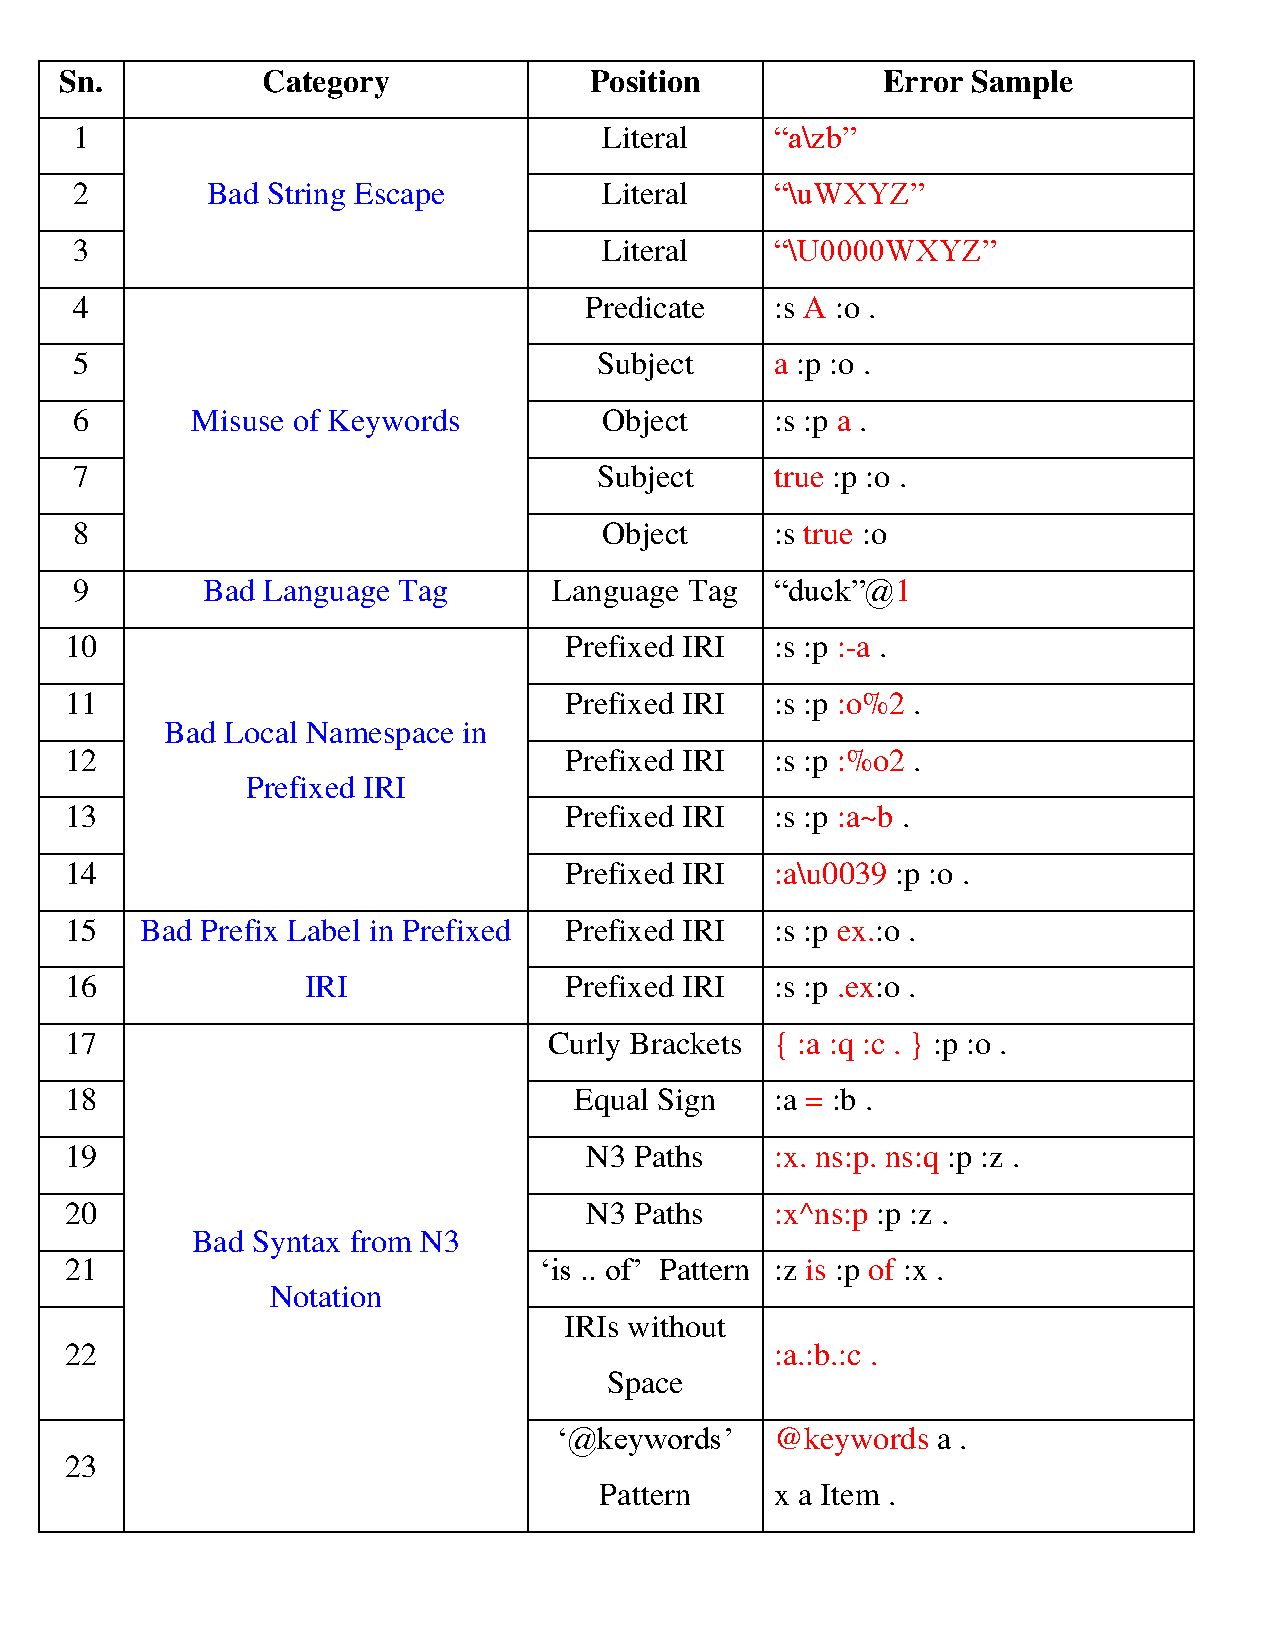
\includegraphics[width=5.5in]{images/firstPageBigTable.pdf}
\end{table}

\includepdf[pages=2-3,pagecommand={},width=\textwidth,noautoscale=true,offset=80 30]{images/bigTable.pdf}
\end{appendices}
